\documentclass[12pt]{article}
\usepackage{nopageno}
\usepackage{amsmath}
\usepackage{amssymb}
\usepackage{amsthm}
\usepackage[left=2cm, right=2cm, top=2cm]{geometry}
\usepackage{enumitem}
\usepackage{graphicx}
\usepackage{caption}
\usepackage{color}   %May be necessary if you want to color links
\usepackage{hyperref}
\hypersetup{
    colorlinks=true, %set true if you want colored links
    linktoc=all,     %set to all if you want both sections and subsections linked
    linkcolor=blue,  %choose some color if you want links to stand out
}
\usepackage{bbm}
\usepackage{soul}
\usepackage{tcolorbox}
\usepackage{tikz}
\tcbuselibrary{theorems}
\tcbuselibrary{breakable}

\newtcbtheorem[number within=section]{mythm}{Theorem}%
{colback=green!5,colframe=green!35!black,fonttitle=\bfseries,unbreakable}{th}
\newtcbtheorem[use counter from=mythm]{mydef}{Definition}%
{colback=blue!5,colframe=blue!35!black,fonttitle=\bfseries,unbreakable}{de}
\newtcbtheorem[use counter from=mythm]{myrem}{Remark}%
{colback=white!5,colframe=white!35!black,fonttitle=\bfseries,unbreakable}{re}
\newtcbtheorem[use counter from=mythm]{myex}{Example}%
{colback=orange!5,colframe=orange!35!black,fonttitle=\bfseries,unbreakable}{ex}
\newtcbtheorem[use counter from=mythm]{myprop}{Proposition}%
{colback=green!5,colframe=green!35!black,fonttitle=\bfseries,unbreakable}{pr}
\newtcbtheorem[use counter from=mythm]{mylem}{Lemma}%
{colback=green!5,colframe=green!35!black,fonttitle=\bfseries,unbreakable}{le}
\newtcbtheorem[use counter from=mythm]{mycor}{Corollary}%
{colback=green!5,colframe=green!35!black,fonttitle=\bfseries,unbreakable}{co}
\newtcbtheorem[]{myprob}{Problem}%
{colback=green!5,colframe=green!35!black,fonttitle=\bfseries,breakable}{pr}

\newcommand{\R}{\mathbb{R}}
\newcommand{\N}{\mathbb{N}}
\newcommand{\Z}{\mathbb{Z}}
\newcommand{\Q}{\mathbb{Q}}
\newcommand{\C}{\mathbb{C}}
\newcommand{\inv}{^{-1}}

\renewcommand*{\proofname}{Solution}
\renewcommand\qedsymbol{$\blacklozenge$}

\setcounter{tocdepth}{3}
\setlength\parindent{0pt}
\hyphenpenalty 10000

\title{CO 380 Course Notes - Spring 2022}
\author{Max Zhu}

\begin{document}
	\maketitle
	\tableofcontents\newpage
	
    \section{Lecture 1: 2022-05-02}
    \begin{myprob}{}{}
        How many ``different-looking'' 2x2x6 solids can be made from 1x1x2 blocks?

        \begin{center}
            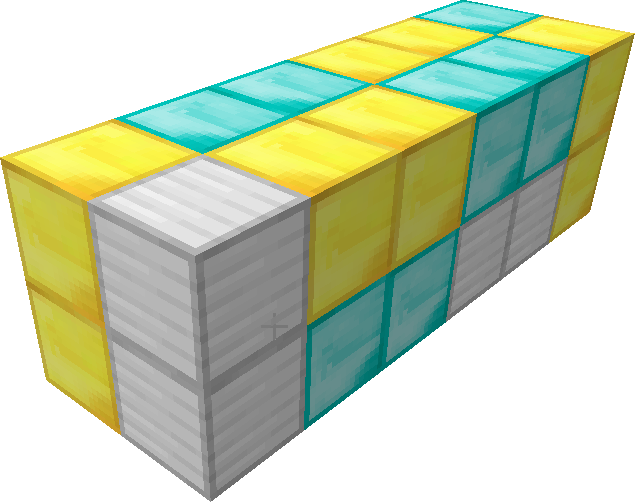
\includegraphics[width=0.5\textwidth]{Fig1.png}
            \captionof{figure}{A rendering of one possible 2x2x6 solid.}
        \end{center}
    \end{myprob}

    \begin{myrem}{}{}
        For the purposes of these problems, \underline{different-looking} means each block is indistinguishable, and rotations and reflections are counted as distinct solids.\\

        We will return to this problem after looking at some simpler problems. For now, consider two dimensions instead of three.
    \end{myrem}

    \begin{myprob}{}{}
        How many ``different-looking'' 2x6 rectangles can be made from 1x2 rectangles?
        \begin{center}
            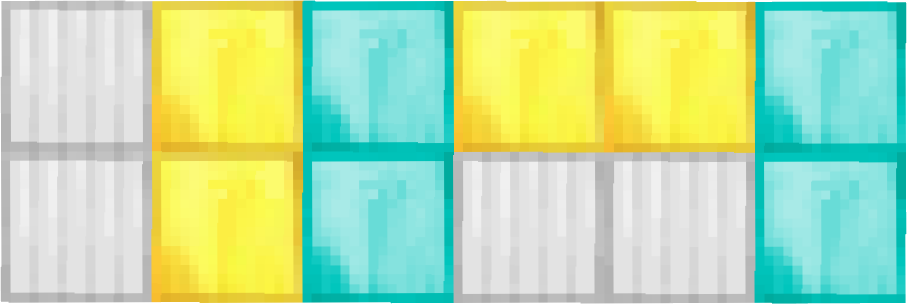
\includegraphics[width=0.5\textwidth]{Fig2.png}
            \captionof{figure}{A rendering of one possible 2x6 rectangle.}
        \end{center}
        Two solutions are given.
        \begin{proof}[Solution 1]
            We can count the number of horizontal blocks. If there is a horizontal block somewhere in the rectangle, there must be a corresponding horizontal block below or above it, since the squares below or above the horizontal block cannot be occupied by vertical blocks.
            
            \begin{center}
                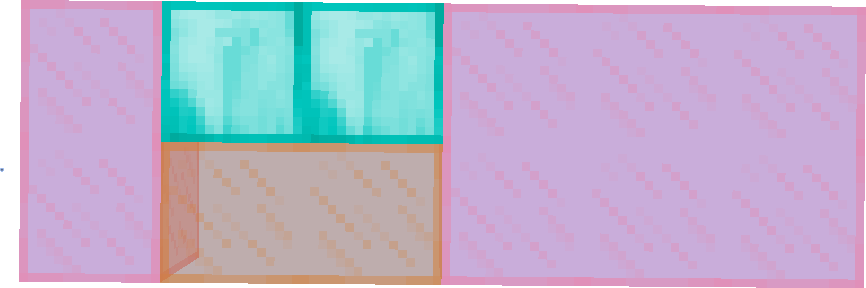
\includegraphics[width=0.5\textwidth]{Fig3.png}
                \captionof{figure}{A horizontal block forces the blocks below or above it to be horizontal.}
            \end{center}

            Furthermore, a horizontal block cannot be above or below two different horizontal blocks, because if it were then that would force an alternating pattern to continue forever, which is impossible.
            
            \begin{center}
                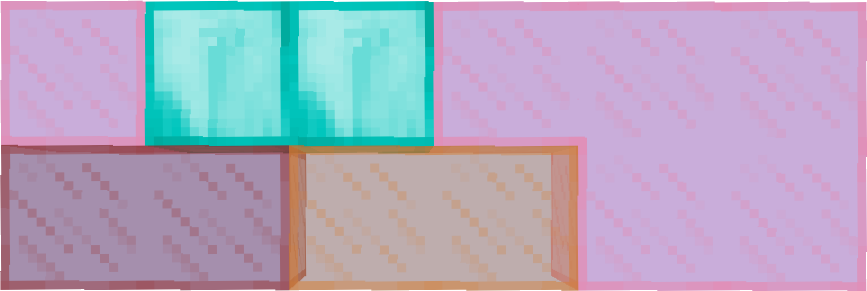
\includegraphics[width=0.5\textwidth]{Fig4.png}
                \captionof{figure}{Two horizontal blocks cannot be ``askew''.}
            \end{center}

            Therefore, all horizontal blocks have a corresponding horizontal block above or below it. So, we can simply consider one row, and count the number of ways horizontal blocks may be placed in it. By brute force counting, we find:
            \begin{itemize}
                \item 1 way to have no horizontal blocks.
                \item 5 ways to have one horizontal block.
                \item 6 ways to have two horizontal blocks.
                \item 1 ways to have three horizontal blocks.
            \end{itemize}
            so the answer is 13.
        \end{proof}

        \begin{proof}[Solution 2]
            We can apply the solution of Problem \ref{pr:3} to $n=6$ to obtain $13$.
        \end{proof}
    \end{myprob}

    \begin{myprob}{}{3}
        If $n\geq1$, how many ways are there of tiling a 2$\times n$ rectangle with 1x2 tiles?

        \begin{proof}
            Let $f(n)$ represent the number of ways to tile a 2$\times n$ rectangle with 1x2 tiles. We first break the set of tilings into two mutually exclusive and exhaustive cases: either the top left square is in a vertical block, or it is in a horizontal block. So, the total number of tilings is equal to the sum of the number of tilings in each case.\\

            Suppose the top left square is in a vertical block. Then, the rest of the rectangle is a 2$\times n-1$ rectangle. Therefore, for this case there are $f(n-1)$ tilings.\\

            Suppose the top left square is in a horizontal block. Then, the squares directly below this block must also be in a horizontal block, and the rest of the rectangle is a 2$\times n-2$ rectangle. Therefore, for this case there are $f(n-2)$ tilings.\\

            Thus, we have $f(n)=f(n-1)+f(n-2)$. Now, to properly define the formula we also need a base case: we can easily check that $f(0)=1$ and $f(1)=1$. Note: We consider $f(0)=1$ because there is exactly $1$ way to fill no space.
        \end{proof}
    \end{myprob}

    \begin{myrem}{}{}
        In the solution of Problem \ref{pr:3}, $f$ is the Fibonacci sequence which starts $1, 1, 2, 3, 5, 8, 13, 21, 34, \dots$. This sequence has a closed form formula for $n\geq1$:
        \begin{align*}
            f(n)&=\frac{1}{\sqrt{5}}\left(\left(\frac{1+\sqrt{5}}{2}\right)^n-\left(\frac{1-\sqrt{5}}{2}\right)^n\right)
        \end{align*}

        A closed form solution is not required in general.
    \end{myrem}

    \newpage
    \section{Lecture 2: 2022-05-04}
    \begin{myprob}{}{}
        If $n\geq1$, how many ways are there of tiling a 3$\times n$ rectangle with 1x3 tiles?

        \begin{proof}
            Let $f(n)$ represent the number of tilings of a 3$\times n$ rectangle with 1x3 tiles. Similar to Problem \ref{pr:3}, we consider two cases. Either the top left square is in a vertical block, or it is in a horizontal block. If the top left square is in a horizontal block, as before it forces the squares below it to also be in horizontal blocks. Thus we have a 3$\times n-3$ rectangle, and there are $f(n-3)$ tilings of this type. If the top left square is in a vertical block, we have a 3$\times n-1$ rectangle, and there are $f(n-1)$ tilings of this type. So we have $f(n)=f(n-1)+f(n-3)$. For base cases, we have $f(0)=1$, $f(1)=1$, $f(2)=1$.
        \end{proof}
    \end{myprob}

    \begin{myprob}{}{}
        If $n\geq1$, how many ways are there of tiling a 3$\times n$ rectangle with 1x2 tiles?

        Two solutions are given. 
        \begin{proof}[Solution 1]
            Let $f(n)$ represent the number of tilings of a 3$\times n$ rectangle with 1x2 tiles. First, note that if $n$ is odd then there is no way to tile the rectangle, as 3 times any odd number is odd, and the 1x2 blocks contain 2 squares. So we may assume $n$ is even.\\

            We break the set of tilings into two cases: either the two leftmost columns are covered by three horizontal tiles, or not.\\

            Suppose the two leftmost columns are covered by three horizontal tiles. Then the rest of the rectangle is a 3$\times n-2$ rectangle, and thus there are $f(n-2)$ tilings covered by this case.
            
            \begin{center}
                
\includegraphics[width=0.5\textwidth]{Fig5.png}
                \captionof{figure}{The leftmost two columns covered by three horizontal tiles.}
            \end{center}

            Now, suppose the two leftmost columns are not covered by three horizontal tiles. Consider the leftmost column: there must be a vetical tile somewhere in the leftmost column because if not, that means the two leftmost columns are covered by three horizontal tiles, which we are assuming is not the case. Since the columns are 3 high, there must be both a vertical and a horizontal block covering the leftmost column. The horizontal block must not be in the middle, as that would force all three blocks to also be horizontal. So, the left side of the rectangle must be in one of these configurations:
            
            \begin{center}
                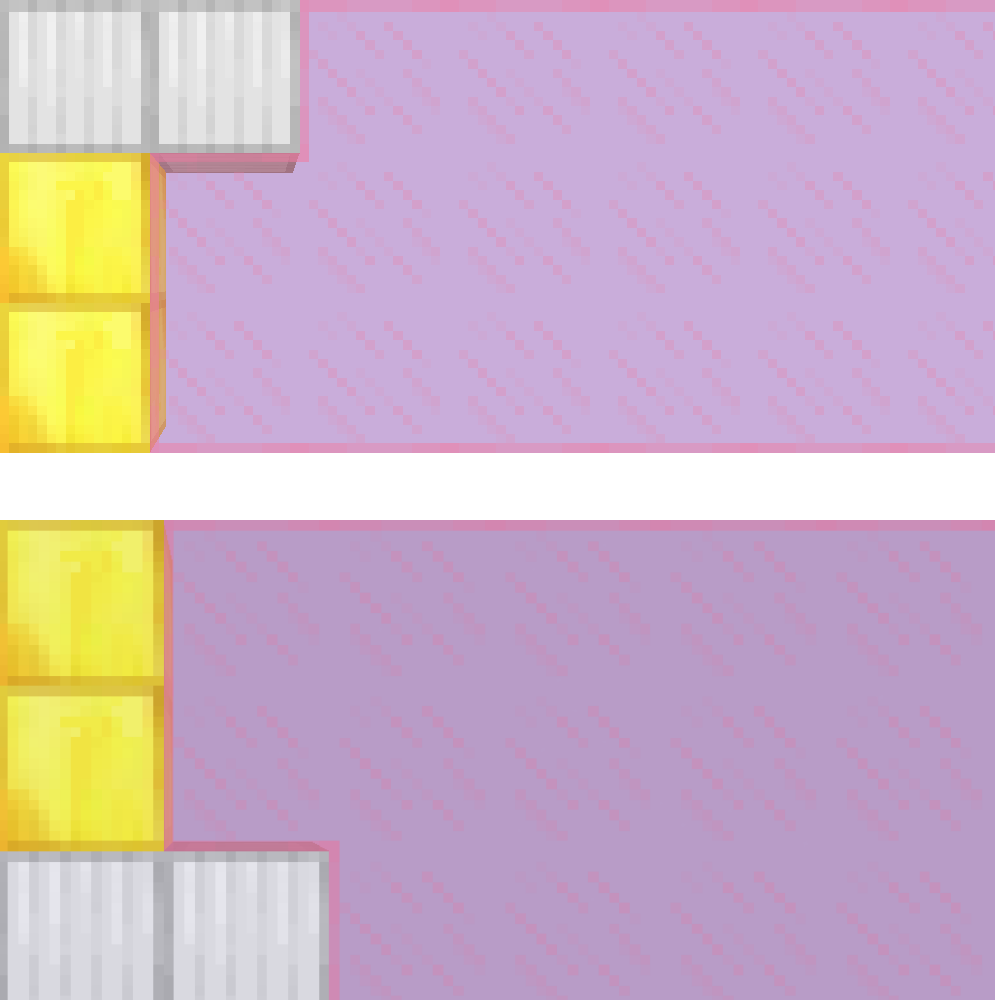
\includegraphics[width=0.5\textwidth]{Fig6.png}
                \captionof{figure}{The two possible configurations.}
            \end{center}

            Since these cases are symmetrical, we consider only the first configuration and multiply our final answer by 2. Now, what remains to be tiled is a 3$\times n-2$ rectangle with an extra two squares sticking out the side.\\
            
            If we tile the extra squares with a vertical block, then we have $f(n-2)$ ways of tiling the remaining 3$\times n-2$ rectangle. If we tile the extra squares with two horizontal blocks, that forces another horizontal block above those horizontal blocks, and we have a similar situation as before, a 3$\times n-4$ rectangle with an extra two squares sticking out the side.
            
            \begin{center}
                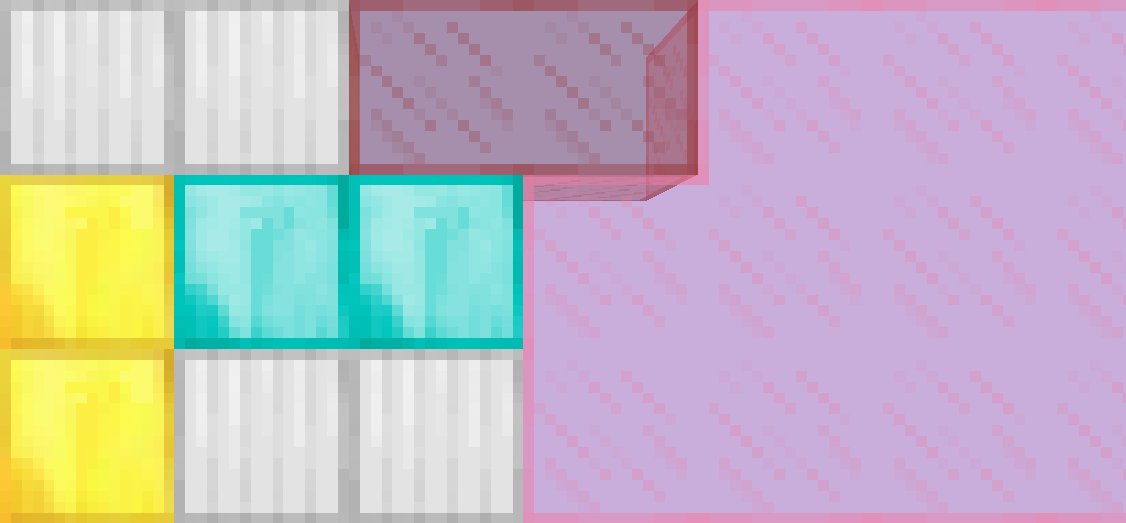
\includegraphics[width=0.5\textwidth]{Fig7.png}
                \captionof{figure}{A 3$\times n-4$ rectangle with an extra two squares sticking out the side.}
            \end{center}

            Eventually, we will use a vertical block to tile the two extra squares. As long as we keep choosing to tile the extra two squares with horizontal blocks, we will come across this configuration. Suppose we choose to use horizontal blocks $i$ times before using a vertical block to tile the two extra squares. Then $i$ can range from $0$ to $\frac{n}{2}-1$, and we are left with a 3$\times n-(2i+2)$ rectangle. Thus the number of tilings in this case are
            \begin{align*}
                2\sum_{i=0}^{\frac{n}{2}-1}f(n-(2i+2))
            \end{align*}

            and our final formula is
            \begin{align*}
                f(n-2)+2\sum_{i=0}^{\frac{n}{2}-1}f(n-(2i+2))=f(n-2)+2(f(n-2)+f(n-4)+\dots+f(2)+f(0))
            \end{align*}

            For our base cases, we have $f(0)=1$, $f(2)=3$.
        \end{proof}
        \begin{proof}[Solution 2.]
            Let $f(n)$ represent the number of tilings of a 3$\times n$ rectangle with 1x2 tiles, and let $g(n)$ represent the number of tilings of a 3$\times n+1$ rectangle with a corner square missing (alternatively, a 3$\times n$ rectangle with two extra squares on the left, one of which is in the middle).\\

            We again break the set of tilings into two cases: either the two leftmost columns are covered by three horizontal tiles, or not.\\

            Suppose the two leftmost columns are covered by three horizontal tiles. Then the rest of the rectangle is a 3$\times n-2$ rectangle. There are 3 ways to tile the two leftmost columns with three horizontal tiles, and thus there are $3f(n-2)$ tilings covered by this case.\\

            Now, suppose the two leftmost columns are not covered by three horizontal tiles. Then as shown in Solution 1 there must be a vertical tile in the leftmost column, which forces a horizontal column in the leftmost column as well. There are two different spots where the vertical block may be. We are left with a shape whose number of tilings is counted by $g(n-2)$. Thus we have the formula $f(n)=3f(n-2)+2g(n-2)$.\\

            Now, consider $g(n)$. It is possible that the two extra squares are covered by a single vertical block; this case would count $f(n)$ tilings by definition. Otherwise, they must be covered by two horizontal blocks, which forces another horizontal block at the top (see Figure 7). We are left with a shape whose tilings are counted by $g(n-2)$. Thus, we have the formula $g(n)=f(n)+g(n-2)$.\\

            For our base cases, we have $f(0)=1$, $g(0)=1$.
        \end{proof}
    \end{myprob}

    \newpage
    \section{Lecture 3: 2022-05-09}
    \begin{myprob}{}{}
        Connie has some gold bars, all of different masses. She gives the 24 lightest bars, which make up $45\%$ of the total mass, to Brennan. She gives the 13 heaviest bars, which make up $26\%$ of the total mass, to Maya. She gives the rest of the bars to Blair. How many bars did Blair receive?

        \begin{proof}
            Let $n$ be the number of bars Blair received.\\
            
            Since Brennan received 24 bars which made up $45\%$ the total mass, the average mass of Brennan's bars is $\frac{45}{24}\%$ of the total. Since Maya received 13 bars which made up $26\%$ of the total mass, the average mass of Maya's bars is $\frac{26}{13}\%$ of the total. The average mass of Blair's bars is $\frac{100-26-45}{n}\%=\frac{29}{n}\%$ of the total.\\

            Now, Brennan received the lightest bars and Maya received the heaviest bars, meaning the average mass of Blair's bars is greater than the average mass of Brennan's bars and also the average mass of Maya's bars is greater than the average mass of Blair's bars. Therefore we have
            \begin{align*}
                \frac{45}{24}&<\frac{29}{n}<\frac{26}{13}\\
                \Longrightarrow n&<\frac{29(24)}{45}\\
                &=15.4\overline{66}\\
                \frac{29(13)}{26}&<n\\
                14.5&<n
            \end{align*}
            Since $n$ is an integer, we have $n=15$.
        \end{proof}
    \end{myprob}

    \begin{myprob}{}{}
        There are 3 pumpkins, which are weighed 2 at a time in each possible combination. The pairs weigh 12, 13, and 15kg. What is the mass of the lightest pumpkin?
        
        \begin{proof}
            Let $a, b, c$ represent the weights of the pumpkins with $a\leq b\leq c$. We have
            \begin{align*}
                a+b&=12\\
                a+c&=13\\
                b+c&=15
            \end{align*}
            since the lightest two pumpkins must be the lightest pair, and the heaviest two pumpkins must be the heaviest pair. So,
            \begin{align*}
                (b+c)-(a+c)&=15-13\\
                b-a&=2\\
                b&=a+2\\
                (b+c)-(a+b)&=15-12\\
                c-a&=3\\
                c&=a+3
            \end{align*}
            So the total mass of the 3 pumpkins is $a+(a+2)+(a+3)$. Also, we have
            \begin{align*}
                (a+b)+(a+c)+(b+c)&=12+13+15\\
                2(a+b+c)&=40\\
                a+b+c&=20
            \end{align*}
            so the total mass is $20$. Equating the two:
            \begin{align*}
                20&=a+(a+2)+(a+3)\\
                &=3a+5\\
                a&=5
            \end{align*}
            So the lightest pumpkin weighs 5kg.
        \end{proof}
    \end{myprob}

    \begin{myprob}{}{}
        Determine positive integers $x, y$ such that $x\leq 5$ and $x^2-2y^2=1$.
        
        \begin{proof}
            We can use trial and error since the number of possible values of $x$ is small.
            \begin{align*}
                x=1\Longrightarrow 1^2-2y^2&=1\text{ so $y=0$ which is not a positive integer.}\\
                x=2\Longrightarrow 2^2-2y^2&=1\text{ so $y=\sqrt{3/2}$ which is not a positive integer.}\\
                x=3\Longrightarrow 3^2-2y^2&=1\text{ so $y=4$ which is a positive integer.}\\
            \end{align*}
            We find that $x=3, y=2$ works.
        \end{proof}
    \end{myprob}

    \begin{myprob}{}{}
        Determine all real numbers $x, y$ such that $5x^2-2xy+2y^2-2x-2y+1=0$.
        
        \begin{proof}
            We rearrange the equation in a form which is a quadratic function in terms of $x$:
            \begin{align*}
                5x^2+(-2y-2)x+(2y^2-2y+1)&=0
            \end{align*}
            Finding the discriminant of this function, we have
            \begin{align*}
                (-2y-2)^2-4(5)(2y^2-2y+1)&=-36y^2+48y-16\\
                &=-4(9y^2-12y+4)\\
                &=-4(3y-2)^2
            \end{align*}
            Now, in order for the equation to have a real solution, the discriminant must be non-negative. This is only possible when $3y-2=0$ because otherwise the discriminant will be negative. Thus we have $y=\frac{2}{3}$ being the only solution. Substituting into the original equation, we find $x=\frac{1}{3}$.
        \end{proof}
    \end{myprob}
\end{document}